
\chapter{Sequences and series of functions}

\lettrine{A}{nalogously} to sequences of numbers we can consider a sequence of functions \(f_0(x),f_1(x), f_2(x), f_3(x),\) etc.
Often it is convenient to write such a sequence as \(\{ f_n(x)\}_{n\in \mathbb{N}}\).
For example, the following are sequences of functions.
\begin{itemize}
  \item \(f_1(x) = x^2, f_2(x)=x^4, f_3(x)=x^6,\ldots \)
  \item \(f_1(x) = e^x, f_2(x)=e^{2x}, f_3(x)=e^{3x},\ldots \)
  \item \(f_n(x) = n \exp \left( - \frac{1}{2}n^2 x^2 \right)\)
\end{itemize}

Note that in the first case we could have instead written \(f_n(x) = x^{2n}\) and in the second case we could have written  \(f_n(x) = e^{nx}\).
The natural number \(n\) is called the index.
Typically the index of the sequence starts from \(n=0\) or \(n=1\) but that's not essential.
The index doesn't need to be \(n\), any other letter, or indeed symbol, can be used.


\section{Convergence and continuity}

We start by recalling the notion of convergence for sequences of numbers.

\begin{definition}
  A sequence of numbers  \(a_1, a_2, a_3,\ldots \) is said to \emph{converge} to \(a\) if, for each \(\epsilon>0\), exists \(N\in \mathbb{N}\) such that \(|a_n - a| < \epsilon\) whenever \(n\geq N\).
\end{definition}
%
\noindent
If a sequence \({\{a_n\}}_{n}\) converges to \(a\) then we write \(a_n \to a\) (as \(n\to \infty\)).
For sequences of functions we will need to consider two different notions of convergence.
In order to understand this difficulty let us consider the following example.

\begin{example*}
  Consider the sequence \(f_n(x) = x^n\) for \(x\in (0,1)\).
  For each \(x\in (0,1)\) we see that \(f_n(x) \to 0\).
  On the other hand, for each \(n\), \(2^{\frac{1}{n}}\in (0,1)\) and \(f_n(2^{\frac{1}{n}}) = \frac{1}{2}\).
\end{example*}


\begin{figure}
  \begin{center}
    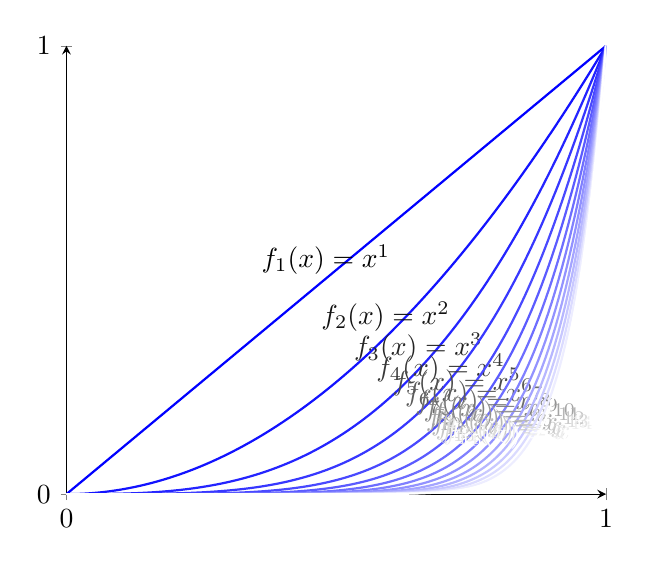
\begin{tikzpicture}
      \begin{axis}[
          axis y line = left,
          axis x line = bottom,
          xtick       = {0,1},
          xticklabels = {$0$,$1$},
          ytick       = {0,1},
          yticklabels = {$0$,$1$},
          samples     = 160,
          domain      = 0:1,
          xmin = 0, xmax = 1,
          ymin = 0, ymax = 1,
        ]
        \foreach[evaluate=\n as \redfrac using (\n-1)*100/(15-1)] \n in {1,...,15}{
            \edef\temp{
              \noexpand\addplot[white!\redfrac!blue, thick, mark=none, text = black] {x^\n} node[pos=0.5, above left] (mid) {};
              \noexpand\node[white!\redfrac!black] at (mid) {$f_{\n}(x) = x^{\n}$};
            }
            \temp
          }
      \end{axis}
    \end{tikzpicture}
    \caption{The sequence of functions \(f_n(x)= x^n\).}
  \end{center}
\end{figure}

\noindent
Up until now we haven't mentioned the domain of the functions in the sequence but to proceed we need to be make this detail rigorous.
We will write that ``\({\{f_n(x)\}}_{n}\) is a sequence of functions on \(D\subset \bR\)'' to mean that there is a fixed \(D\subset \bR\) and, for each \(n\in \bN\), \(f_{n}\) is a function with domain \(D\) (i.e., \(f_n : D \to \bR\)).


\begin{definition}[pointwise convergence]
  Let \(D\subset \mathbb{R}\),
  let \(f_n(x)\) be a sequence of functions on \(D\)
  and let \(f(x)\) be a function on \(D\).
  If \(f_n(x) \to f(x)\) for each \(x\in D\) we say that \(f_n\) is \emph{pointwise convergent} to \(f\).
\end{definition}

\begin{definition}[uniform convergence]
  Let \(f_n(x)\) be a sequence of functions on \(D\subset \mathbb{R}\)
  and let \(f(x)\) be a function on \(D\).
  If, for each \(\epsilon>0\), there exists \(N\) such that for every \(n\geq N\) and every \(x\in D\), \(|f_n(x) - f(x)| < \epsilon\) then we say that \(f_n\) is \emph{uniformly convergent} to \(f\).
\end{definition}

\noindent
\textbf{Problem:}
Show that the sequence \(f_n(x) = x^n\) converges uniformly on \((0,\frac{1}{2})\).

\noindent
\textbf{Solution:}
We observe that it converges pointwise to the constant function \(f(x)=0\).
\begin{itemize}
  \item We also observe that \(|f_n(x) - f(x) | \leq \frac{1}{2^n}\) for all \(x\in (0,\frac{1}{2})\).
  \item This means that, for every \(\epsilon>0\), if we can choose \(N=-\log_{2}\epsilon\) then \(|f_n(x) - f(x) | \leq \epsilon\) whenever \(n\geq N\).
\end{itemize}


\begin{definition}
  Let \(f(x)\) be a functions on \(D\subset \mathbb{R}\).
  We say that \(f\) is \emph{continuous} at \(p\in D\) if, for each \(\epsilon>0\), there is \(\delta >0\) such that \(|f(x)-f(p)| <\epsilon\) whenever \(x\in D\), \(|x-p| <\delta\).
  We say that \(f\) is \emph{continuous on \( D\)} if \(f\) is continuous at every \(p\in D\).
\end{definition}




\begin{figure}
  \begin{center}
    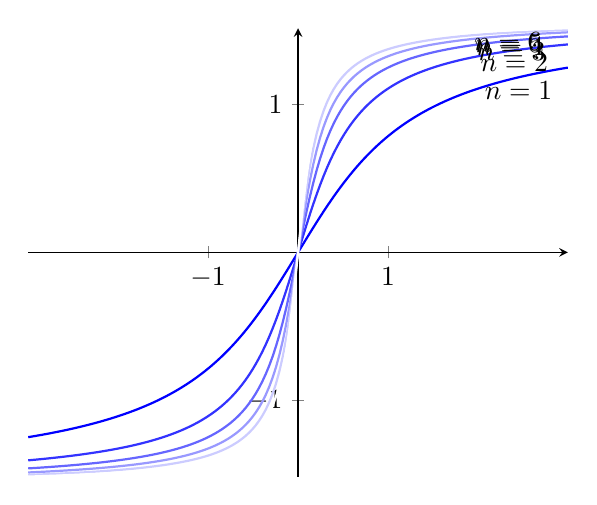
\begin{tikzpicture}
      \begin{axis}[
          axis y line = center,
          axis x line = center,
          xtick       = {-1,0,1},
          xticklabels = {$-1$,$0$,$1$},
          % ytick       = {-1,0,1},
          % yticklabels = {$-1$,$0$,$1$},
          samples     = 160,
          domain      = -3:3,
          xmin = -3, xmax = 3,
          % ymin = 0, ymax = 1,
        ]
        \foreach[evaluate=\n as \redfrac using (\n-1)*100/(6-1)] \n in {1,...,6}{
            \edef\temp{
              \noexpand\addplot[white!\redfrac!blue, thick, mark=none, text = black] {atan(x*\n)*pi/180} node[pos=0.9, below right] (mid) {};
              \noexpand\node[black] at (mid) {$n =\n$};
            }
            \temp
          }
      \end{axis}
    \end{tikzpicture}
    \caption{The sequence of functions \(f_n(x)= \arctan(nx)\).}
  \end{center}
\end{figure}

It is natural to consider a sequence of continuous functions which converge and ask if the function they converge to is continuous.
What about the sequence of functions \(f_n(x) = \arctan (nx)\)?

\begin{theorem}
  \label{thm:continuous-limit}
  Suppose that \(f_n \to f\) uniformly on \(D\) and that the \(f_n\) are continuous on \(D\).
  Then \(f\) is continuous on \(D\).
\end{theorem}


\begin{proof}
  Let \(p\in D\).
  Uniform convergence means that, for each \(\epsilon>0\), there exists \(N\) such that for every \(n\geq N\) and every \(x\in D\), \(|f_n(x) - f(x)| < \frac{\epsilon}{3}\).
  By continuity of \(f_N(x)\) at \(x=p\), there is a \(\delta >0\) such that \(|f_N(x)-f_N(p)| < \frac{\epsilon}{3} \) whenever \(x\in D\), \(|x-p| <\delta\).
  Since
  \[
    | f(x) - f(p) | = |f(x) - f_N(x) + f_N(x) - f_N(p) + f_N(p) - f(p) | \]
  this means that, for all \(|x-p| <\delta\),
  \[
    \begin{aligned}
      | f(x) - f(p) | & \leq   |f(x) - f_N(x)| + |f_N(x) - f_N(p)| + |f_N(p) - f(p) | \\
                      & < 3 \frac{\epsilon}{3} = \epsilon.
    \end{aligned}
  \]
  This proves the continuity of \(f\) at \(p\). Since \(p\in D\) is arbitrary this shows the continuity of \(f\) on \(D\).
\end{proof}


Recall that integrals are defined rigorously using the notion of a step functions.

\begin{theorem}
  \label{thm:limit-of-integral}
  Suppose that \(f_n\) are continuous functions on \([a,b] \subset \mathbb{R}\), uniformly convergent to \(f\).
  Then
  \[
    \lim_{n\to \infty} \int_{a}^{b} f_n(x) \ dx = \int_{a}^{b} f(x) \ dx.
  \]
\end{theorem}

\begin{proof}
  The uniform convergence implies that for each \(\epsilon>0\), there exists \(N\) such that for every \(n\geq N\) and every \(x\in D\), \(|f_n(x) - f(x)| <  \frac{\epsilon}{b-a}\).
  This means that
  \[ \Big| \int_{a}^{b} f_n(x) \ dx - \int_{a}^{b} f(x) \ dx \Big|
    \leq \int_{a}^{b} | f_n(x) - f(x) | \ dx
    \leq (b-a) \frac{\epsilon}{b-a} = \epsilon.\]
  This shows that \(\int_{a}^{b} f_n(x) \ dx \to  \int_{a}^{b} f(x) \ dx\).
\end{proof}


\subsection*{Series of functions}



Recall that for a sequence \({\{a_n\}}_{n}\) of numbers,
the series \(\sum_{n}a_n\) is the sequence \({\{\sum_{k=1}^{n}a_k\}}_{n}\) of numbers (the partial sums).
We say that the series  \(\sum_{n}a_n\) is convergent if \({\{\sum_{k=1}^{n}a_k\}}_{n}\) is convergent.



\begin{definition}
  Let \(\{f_n\}\) be a sequence of functions.
  We say that the series \(\sum_{n} f_n\)
  \begin{itemize}
    \item   is \emph{pointwise convergent} if
          \(\sum_{k=1}^{n} f_k(x)\) is pointwise convergent,
    \item   is \emph{uniformly convergent} if
          \(\sum_{k=1}^{n} f_k(x)\) is uniformly convergent.
  \end{itemize}
\end{definition}


\begin{theorem}
  Suppose that the series \(\sum_{n} f_n\) is uniformly convergent to \(g\) on \(D\) and the \(f_n\) are continuous on \(D\).
  Then \(g\) is continuous on \(D\).
\end{theorem}


\begin{proof}
  If the \(f_k\) are continuous then the \(\sum_{k=1}^{n} f_k\) are continuous.
  This means that Theorem~\ref{thm:continuous-limit} applies.
\end{proof}



\begin{theorem}
  Suppose that the series \(\sum_{n} f_n\) is uniformly convergent to \(g\) and the \(f_n\) are continuous.
  Then
  \[
    \lim_{n\to\infty} \int_{a}^{b}  \sum_{k=1}^{n} f_k(x)  \ dx = \int_{a}^{b} g(x) \ dx.
  \]
\end{theorem}


\begin{proof}
  Again, that the \(f_k\) are continuous means that the \(\sum_{k=1}^{n} f_k\) are continuous.
  This means that Theorem~\ref{thm:limit-of-integral} applies.
\end{proof}


Here and subsequently it is convenient to recall three commons tests which are useful for proving convergence:
\href{https://en.wikipedia.org/wiki/Ratio_test}{ratio test},
\href{https://en.wikipedia.org/wiki/Root_test}{root test},
\href{https://en.wikipedia.org/wiki/Direct_comparison_test}{comparison test}.
%
For series of functions we have the following test for convergence.

\begin{theorem}[Weierstrass M-test]
  Suppose that \({\{f_n\}}_n\) is a sequence of functions on \(D\), that \({\{M_n\}}_n\) is a sequence of positive numbers
  and that \(|f_n(x)|\leq M_n\).
  If the series \(\sum_{n=0}^{\infty}M_n\) is convergent then the series \(\sum_{n=0}^{\infty}f_n\) is uniformly convergent.
\end{theorem}



\begin{proof}
  By the comparison test \(\sum |f_n(x)| \) is convergent for all \(x\in D\).
  I.e., for each \(x\) the series \(\sum f_n(x) \) is absolutely convergent and so we let \(f(x)\) be the limit.
  We compute
  \[
    \Big|f(x) - \sum_{k=1}^{n} f_k(x)  \Big|
    =
    \Big|\sum_{k=n+1}^{\infty} f_k(x)  \Big|
    \leq \sum_{k=n+1}^{\infty} |f_k(x)|
    \leq  \sum_{k=n+1}^{\infty} M_k.
  \]
  As \(\sum_{n}M_n\) is convergent this last expression tends to \(0\) as \(k\to \infty\).
  This estimate is independent of \(x\).
\end{proof}




\section{Power series}



\begin{definition}
  Let \({\{a_n\}}_{n}\) be a series of numbers.
  The series
  \(\sum_{n} a_n x^n\)
  is called a \emph{power series}.
\end{definition}
Typically the power series will converge for some \(x\) and diverge for other \(x\).
Note that we could permit \(x\) to be a complex number and the entire work of this section holds verbatim.
However, for the present purposes we will assume that \(x \in \bR\) and that the coefficients \(a_n \in \bR\).

\begin{example*}
  Let \(a_n = 2^{-n}\).
  The power series \(\sum_{n} a_n x^n = \sum_{n}\frac{x^n}{2^n}\) is convergent when \(\abs{x}<2\) and divergent  when \(\abs{x} > 2\).
  To see this we apply the root test and observe that  \(\lim_{n\to\infty}\big(\frac{\abs{x}^n}{2^n} \big)^{\frac{1}{n}}=\frac{\abs{x}}{2}\).
\end{example*}

\begin{example*}
  Let \(a_n = \frac{1}{n!}\).
  The power series \(\sum_{n}\frac{x^n}{n!}\) is convergent for all \(x\).
  To see this we use the ratio test and observe that  \(\abs{\frac{x^{n+1}}{(n+1)!} }/ \abs{\frac{zx^n}{n!}} = \frac{\abs{x}}{n+1}\) and that \(\lim_{n\to\infty} \frac{\abs{x}}{n+1} = 0 \) for any \(x\).
\end{example*}



\section{Radius of convergence}

A key notion is determining exactly the domain on which a power series converges.

\begin{theorem}[uniformly convergent power series]
  Suppose that \(\sum_{n}a_n x^n\) converges for some \(x=x_0 \neq 0\).
  Let \(R<\abs{x_0}\).
  Then the series is uniformly and absolutely convergent for all \(x\) such that \(\abs{x}\leq R\).
\end{theorem}

\begin{proof}
  \begin{itemize}
    \item \(\sum_n a_n x_0^n\) is convergent \(\implies\) for all \(n\), \(\abs{a_n x_0^n} \leq M\) for some \(M>0\);
    \item \(\abs{a_n x^n} = \abs{a_n x_0^n} \cdot \abs{\frac{x}{x_0}}^n \leq M \frac{R^n}{\abs{x_0}^n}\);
    \item \(\sum_n M \frac{R^n}{\abs{x_0}^n}\) is a geometric sum and so convergent;
    \item M-test \(\implies\) series is uniformly and absolutely convergent when \(\abs{x}\leq R\).  \qedhere
  \end{itemize}
\end{proof}




\begin{theorem}[radius of convergence]
  Suppose exists  \(x_1,x_2 \neq 0\) such that \(\sum_n a_n x_1^n\) is convergent and \(\sum_n a_n x_2^n\) is divergent.
  Then exists \(r>0\) such that \(\sum_n a_n x^n\) is convergent for \(\abs{x}<r\) and divergent for \(\abs{x}>r\).
\end{theorem}

\begin{proof}
  \begin{itemize}
    \item Let \(A\) be the set of real numbers for which \(\sum_n a_n x^n\) is convergent;
    \item Let \(r\) be the least upper bound of \(A\);
    \item Series  \(\sum_n a_n x^n\) is convergent whenever \(\abs{x}<r\);
    \item If \(\abs{x}>r\) and \(\sum_n a_n x^n\) is convergent then this contradicts the definition of \(A\) and so  \(\sum_n a_n x^n\) is divergent for \(\abs{x}>r\). \qedhere
  \end{itemize}
\end{proof}


\begin{definition}
  This \(r\) is called the \emph{radius of convergence} for the power series \(\sum_n a_n z^n\).
\end{definition}

We use the following convention:
if \(\sum_n a_n x^n\) converges for all \(x\in \bC\) we say the radius of convergence is \(\infty\);
if \(\sum_n a_n x^n\) doesn't converge except  \(x=0\) we say the radius of convergence is \(0\).

Note: all of the above concerning power series holds verbatim for \(x\) a complex number and so ``radius'' is more meaningful since it truly corresponds to a disk in the complex plane.




\section{Integrating and differentiating power series}



Let \(a_n \in \bR\), \(x\in \bR\).
If \(\sum_n a_n x^n\)converges we define the function \(f(x) = \sum_{n=0}^{\infty} a_n x^n\).

In general exchanging limits with derivatives and integrals is problematic but for power series the situation is good.



\begin{theorem}[integrating power series]
  \label{thm:integrate-power}
  Suppose that, for \(x\in (-r,r)\), the series  \(f(x) = \sum_{n=0}^{\infty} a_n x^n\) is convergent.
  Then \(f(x)\) is continuous and \(\int_0^x f(y) \ dy = \sum_{n=0}^{\infty} \frac{a_n}{n+1} x^{n+1}\).
\end{theorem}

\begin{proof}
  \begin{itemize}
    \item Let \(\abs{x}<R<r\);
    \item Series is uniformly convergent for \(y\in[-R,R]\);
          {Which theorem do we use?}
    \item \(f(x)\) is continuous and so we can interchange limit and integral: % Which theorem do we use?
          \[
            \int_0^x f(y) \ dy
            = \sum_{n=0}^{\infty} \int_0^x  {a_n} x^{n}
            = \sum_{n=0}^{\infty} \frac{a_n}{n+1} x^{n+1}. \qedhere
          \]
  \end{itemize}
\end{proof}





\begin{theorem}[differentiating power series]
  \label{thm:differentiate-power}
  Suppose that, for \(x\in (-r,r)\), the series  \(f(x) = \sum_{n=0}^{\infty} a_n x^n\) is convergent.
  Then \(f(x)\) is differentiable and \(f'(x) =\sum_{n=1}^{\infty} n a_nx^{n-1}\), convergent for \(x\in (-r,r)\).
\end{theorem}



\begin{proof}
  \begin{itemize}
    \item Let \(\abs{x}<R<r\);
    \item
          \(\sum_{n=1}^{\infty} n a_nx^{n-1}    = \sum_{n=1}^{\infty} a_n R^{n} \cdot \frac{n}{R} \cdot \frac{{x}^{n-1}}{R^{n-1}}\);
    \item \(\sum_{n=1}^{\infty} a_n R^n\) is absolutely convergent and \(  \frac{n}{R}  \cdot ( \frac{\abs{x}}{R} )^{n-1}\) is bounded;
    \item \(\sum_{n=1}^{\infty} n a_nx^{n-1} \) is absolutely convergent
          (comparison test);
    \item \(g(x) =\sum_{n=1}^{\infty} n a_nx^{n-1} \) is a power series;
    \item \(\int_0^x g(y) \ dy = \sum_{n=1}^{\infty} a_nx^{n} = f(x) - a_0\) (by Theorem~\ref{thm:integrate-power});
    \item By the fundamental theorem of calculus this concludes the proof. \qedhere
  \end{itemize}
\end{proof}






% \begin{example}[\(\log(x+1)\)]
%   \begin{itemize}
%     \item \(\frac{1}{x+1} = \sum_{n=0}^{\infty}(-1)^{n}x^{n}\) for \(\abs{x}<1\);
%     \item \(\left(\log(x+1)\right)' = \frac{1}{x+1} \);
%     \item \(\log(x+1) =  \sum_{n=0}^{\infty}\frac{(-1)^{n}}{n+1} x^{n+1} \) for \(\abs{x}<1\).
%   \end{itemize}
% \end{example}

% \begin{example}[\(\arctan x\)]
%   \begin{itemize}
%     \item  \(\frac{1}{x^2+1} = \sum_{n=0}^{\infty}(-1)^{n}x^{2n}\) for \(\abs{x}<1\);
%     \item \(\left( \arctan x\right)' = \frac{1}{x^2+1} \);
%     \item \(\arctan(x) =  \sum_{n=0}^{\infty}\frac{(-1)^{n}}{2n+1} x^{2n+1} \) for \(\abs{x}<1\).
%   \end{itemize}
% \end{example}




% \subsection{Exercises}

% \begin{enumerate}
%   \item Determine the radius of convergence \(r\) of the following power series. If \(r\) is finite, test for convergence at the boundary points.
%         \begin{enumerate}
%           \item \(\displaystyle\sum_{n=0}^{\infty}\frac{z^n}{3^n}\),
%           \item \(\displaystyle\sum_{n=0}^{\infty}\frac{(z+3)^n}{(n+1)2^n}\),
%           \item \(\displaystyle\sum_{n=1}^{\infty} \frac{n! z^n}{n^n}\);
%         \end{enumerate}
%         % \item It is known that 
%         %   \( \displaystyle\sum_{n=1}^{\infty}\frac{\cos(nx)}{n^2}=\frac{x^2}{4}-\frac{\pi x}{2}+\frac{\pi^2}{6}\)
%         %   if \(0\leq x \leq \pi\).
%         %   Show that \(\displaystyle\sum_{n=1}^{\infty}\frac{1}{n^2} = \frac{\pi^2}{6}\).
%   \item Let \(f_n(x) = \frac{\sin(nx)}{n}\), \(n\in\bN\). For each fixed \(x\) let \(f(x) = \lim_{n\to\infty}f_n(x)\). Calculate
%         \begin{enumerate}
%           \item \(\lim_{n\to \infty} f_n'(0)\),
%           \item \(f'(0)\).
%         \end{enumerate}
% \end{enumerate}





% \subsection{Exercises}

% \begin{enumerate}
%   \item Calculate the Taylor's series for \(f(x) = e^x\) at \(x=0\).
%   \item Consider the function
%         \[
%           f(x) = \begin{cases}
%             e^{-{1}/{x}} & \text{if \(x > 0\)}    \\
%             0            & \text{if \(x\leq 0\)}.
%           \end{cases}
%         \]
%         \begin{enumerate}
%           \item Is \(f(x)\) infinitely differentiable for every \(x\in \bR\)?
%           \item What is the Taylor's series for \(f(x)\) at \(0\)?
%           \item What is the difficulty?
%         \end{enumerate}
% \end{enumerate}



Let \(a\), \(x\) and the coefficients \(a_n\) be real numbers.
The series
\[
  f(x) = \sum_{n=0}^{\infty} a_n (x-a)^n
\]
defines a function on the interval \((a-r,a+r)\),
where  \(r\)  is the \emph{radius of convergence}.
%
The series is said to \emph{represent} the function \(f\)
and is called the \emph{power series expansion} of \(f\) about \(a\).

Two important questions are: Given the series, what are the properties of \(f\)?
Given a function \(f\), can it be represented by a power series?
Only rather special functions possess power-series expansions however the class of such functions is very useful in practice.



\section{Uniqueness of power series}

The conclusion of Theorem~\ref{thm:differentiate-power} can be iterated and leads to the following result.

\begin{theorem}
  Suppose that \(f(x) = \sum_{n=0}^{\infty} a_n (x-a)^n\) is convergent for \(x\in (a-r,a+r)\).
  Then \(f(x)\) has derivatives of every order and, for \(k\in \bN\),
  \[
    f^{(k)}(x) =\sum_{n=k}^{\infty} n(n-1)\cdots (n-k+1) a_n(x-a)^{n-k}.
  \]
\end{theorem}

The following result is a crucial piece of information about power series and is one major reason why they are useful.

\begin{theorem}[uniqueness of power series]
  \label{thm:unique-power}
  If two power series \(\sum_n a_n(x-a)^n\) and  \(\sum_n b_n(x-a)^n\) are equal in a neighbourhood of \(a\) then the two series are equal term-by-term:
  \(a_n = b_n = \frac{f^{(n)}(a)}{n!}\) for every \(n\in \bN\).
\end{theorem}

\begin{proof}
  \(f^{(k)}(x) = k! a_k + \displaystyle\sum_{n=k+1}^{\infty} n\cdots (n-k+1) a_n(x-a)^{n-k}\)
  so \(f^{(k)}(a) = k! a_k \).
\end{proof}


Suppose that a function \(f(x)\) is infinitely differentiable on an open interval about \(a\).
We consider the \emph{Taylor's series generated by \(f\) at \(a\)}:
\[
  \sum_{n=0}^{\infty} \frac{f^{(n)}(a)}{n!} (x-a)^{n}.
\]
Observe how the coefficients in the Taylor's series coincide with the formula obtained in the above results.
\textbf{Question:}
Does the Taylor's series converge on the entire interval?
In general, no. However we can calculate the radius of convergence of the power series.
\textbf{Question:}
If the Taylor's series converges, is it equal to \(f(x)\) on the interval?
{In general it might not as seen in the following example.}

\begin{example*}
  Let  \(f(x) = e^{-1/x^2}\).
  If we proceed to calculate the Taylor's series about \(x=0\) we obtain:

  \begin{tabular}{ r l  l}
    \(f(x) = \)  & \( \exp(-x^{-2})\)
                 &
    \(f(0)=0\)
    \\
    \(f'(x)=\)   & \( 2x^{-3} \exp(-x^{-2})\)
                 &
    \(f'(0)=0\)
    \\
    \(f''(x)=\)  & \( (-6 x^{-4}   + 4x^{-6} )\exp(-x^{-2})  \)
                 &
    \(f''(0)=0\)
    \\
    \(f'''(x)=\) & \( 4 (2x^{-9} - 9 x^{-7} + 6 x^{-5})\exp(-x^{-2})\)
                 &
    \(f'''(0)=0\)
  \end{tabular}

  \noindent
  The Taylor's series is consequently \(\sum_{n=0}^{\infty} 0 = 0\).
  It does converge but has nothing to do with the original function.
\end{example*}









\section{Power series and differential equations}

In this section we will use some of the strength of power series in a particular application. This is a method which we can use to solve certain power series. The method is best illustrated with an example.
This method of solving differential equations is called the ``Method of undetermined coefficients''.

\noindent
\textbf{Problem:}
Find a function \(y(x)\) which satisfies the differential equation
\[
  (1-x^2)y''(x) = -2y(x)
\]
and satisfies the initial conditions \(y(0)=1\), \(y'(0)=1\).

\noindent
\textbf{Solution:}
We start by assuming that there exists a power series solution \(y(x) = \sum_{n=0}^{\infty}a_nx^n\) convergent for \(x \in (-r,r)\) for some \(r>0\) to be determined later.
\begin{enumerate}
  \item
        By Theorem~\ref{thm:differentiate-power}, \(y'(x) = \sum_{n=1}^{\infty}n a_n x^{n-1}\) and \(y''(x) = \sum_{n=2}^{\infty}n(n-1) a_n x^{n-2}\);
  \item And so
        \[
          \begin{aligned}
            -2 \sum_{n=0}^{\infty}a_nx^n
             & = (1-x^2)y''(x)
            = (1-x^2) \sum_{n=2}^{\infty}n(n-1) a_n x^{n-2}                                        \\
             & = \sum_{n=2}^{\infty}n(n-1) a_n x^{n-2} - \sum_{n=2}^{\infty}n(n-1) a_n x^{n}       \\
             & = \sum_{n=0}^{\infty}(n+2)(n+1) a_{n+2} x^{n} - \sum_{n=0}^{\infty}n(n-1) a_n x^{n}
          \end{aligned}
        \]
  \item Consequently, by Theorem~\ref{thm:unique-power}, \(0 = 2a_n +  (n+2)(n+1) a_{n+2} -  n(n-1) a_n \) for each \(n \in \bN_0\);
  \item Equivalently \(a_{n+2} = \frac{n-2}{n+2}a_n\);
  \item Using the initial conditions,  \(a_0 = y(0) = 1\), \(a_1 = y'(0) = 1\);
  \item For the even coefficients:
        \begin{itemize}
          \item \(a_2 =  \frac{0-2}{0+2}a_0 = -1\),
          \item \(a_4 =  \frac{2-2}{2+2}a_2 = 0\),
          \item  \(a_6 =  \frac{4-2}{4+2}a_4 = 0\),\ldots;
        \end{itemize}
  \item For the odd coefficients:
        \begin{itemize}
          \item \(a_3 =  \frac{1-2}{1+2}a_1 = -\frac{1}{3}\),
          \item \(a_5= \frac{3-2}{3+2}a_3 = \frac{1}{5}(-\frac{1}{3})\),\ldots
          \item \(a_{2n+1} = \frac{1}{(2n+1)(2n-1)}\);
        \end{itemize}
  \item Formally we have the series solution
        \begin{equation}
          \label{eq:sol-diff-eq}
          y(x) = 1 - x^2 + \sum_{n=0}^{\infty} \frac{x^{2n+1}}{(2n+1)(2n-1)},
        \end{equation}
  \item We see that this series is convergent for \(\abs{x}<1\).
\end{enumerate}
%
Consequently we have shown that the function defined above \eqref{eq:sol-diff-eq} is well-defined in the interval \((-1,1)\) and is a solution to the given differential equation.



\subsection*{Suggested further reading}

\begin{itemize}
  \item Apostol, ``Calculus Volume 1'' -- Chapter 11
  \item \href{https://tutorial.math.lamar.edu/Classes/CalcII/SeriesIntro.aspx}{Paul Dawkins' online math notes ``Sequences and Series.''}
\end{itemize}



% \section*{Additional material}


% \subsection*{Error term in Taylor's series}

% We define the error term in \(n\)\textsuperscript{th} approximation as
% \[
%   E_n(x) := f(x) - \sum_{k=0}^{n} \frac{f^{(k)}}{k!}(x-a)^k.
% \]
% Integration by parts implies that
% \[
%   E_n(x) = \frac{1}{n!} \int_{a}^{x} (x-y)^n f^{(n+1)}(y) \ dy.
% \]
% Convergence of the Taylor's series to \(f(x)\) is implied by \(E_n(x) \to 0\) as \(n\to \infty\).




%   {A sufficient condition for convergence of a Taylor's series}

% \begin{theorem}
%   Assume \(f\) is infinitely differentiable on \(I=(a-r,a+r)\) and exists \(A>0\) such that
%   \[
%     \abs{f^{(n)}(x)}\leq A^n, \quad \text{for all \(n\in \bN, x\in I\)}.
%   \]
%   Then Taylor's series generated by \(f\) at \(a\) converges to \(f(x)\) for each \(x\in I\).
% \end{theorem}



% \begin{proof}
%   \[
%     \abs{E_n(x)}
%     \leq \frac{1}{n!} \int_{a}^{x} \abs{x-y}^n A^{n+1}  \ dy
%     \leq \frac{1}{n!} r r^n  A^{n+1} = rA \frac{(rA)^n}{n!}.
%   \]
%   \(\frac{(rA)^n}{n!} \to 0\) as \(n\to \infty\) and so \(\abs{E_n(x)}  \to 0\) as \(n\to \infty\).
% \end{proof}




% \subsection*{Examples of Taylor's series}

% \begin{itemize}
%   \item \(\sin x = x - \frac{x^3}{3!} + \frac{x^5}{5!} - \frac{x^7}{7!} + \ldots + (-1)^{n-1}\frac{x^{2n-1}}{(2n-1)!} + \ldots\),
%   \item \(\cos x = 1 - \frac{x^2}{2!} + \frac{x^4}{4!} - \frac{x^6}{6!} + \ldots + (-1)^{n}\frac{x^{2n}}{(2n)!} + \ldots\),
%   \item \(e^x = 1 + x + \frac{x^2}{2!} + \cdots + \frac{x^n}{n!} + \cdots\)
% \end{itemize}

% Valid on what interval?


%   \subsection{Binomial series}

%   For any \(\alpha \in \bR\), \(n\in \bN\), let
%   \(  \binom{\alpha}{n}:= \frac{\alpha (\alpha-1) \cdots (\alpha-n+1)}{n!}\).


%   \begin{theorem}
%     Let \(\alpha \in \bR\).
%     Then \((1+x)^\alpha = \displaystyle\sum_{n=0}^{\infty} \textstyle\binom{\alpha}{n} x^n\)
%     whenever \(\abs{x}<1\).
%   \end{theorem}



%   \begin{proof}
%     \begin{enumerate}
%       \item By the ratio test the right hand side converges;
%       \item Let \(f(x) = (1+x)^\alpha\);
%       \item \(f'(x) = \alpha(1+x)^{\alpha-1}\) and so \(f(x)\) is a solution to the differential equation
%             \[
%               y'(x) = \frac{\alpha}{x+1}y(x)
%             \]
%             and satisfies the initial condition \(f(0)=1\).
%       \item \(g(x) := \sum_{n=0}^{\infty} \binom{\alpha}{n} x^n\) satisfies the same differential equation and initial condition. \qedhere
%     \end{enumerate}
%   \end{proof}




%   \subsection{Does \(g(x)\) satisfy this differential equation?}

%   First observe that % (recall \(  \binom{\alpha}{n} := \frac{\alpha (\alpha-1) \cdots (\alpha-n+1)}{n!}\))
%   \[
%     (n+1)\binom{\alpha}{n+1} = (\alpha - n)\binom{\alpha}{n}
%     \quad \Longleftrightarrow \quad
%     (n+1)\binom{\alpha}{n+1} + n \binom{\alpha}{n} = \alpha \binom{\alpha}{n}
%     .
%   \]
%   We defined \(g(x) = \sum_{n=0}^{\infty} \binom{\alpha}{n} x^n\)  and so
%   \[
%     g'(x)
%     =  \sum_{n=1}^{\infty} n \binom{\alpha}{n} x^{n-1}
%     =  \sum_{n=0}^{\infty} (n+1) \binom{\alpha}{n+1} x^n.
%   \]
%  ({Dummy variable in sum})
%   Consequently
%   \[
%     \begin{aligned}
%       (1+x)g'(x)
%        & = \sum_{n=0}^{\infty} \left( (n+1)\binom{\alpha}{n+1} + n\binom{\alpha}{n}    \right)  x^n \\
%        & = \alpha  \sum_{n=0}^{\infty} \binom{\alpha}{n}  x^n = \alpha g(x).
%     \end{aligned}
%   \]
%   Additionally \(g(0) = 1\).


